\subsection{How Music is Made}
\par
Sound is produced when something vibrates. The vibration causes the medium around it to vibrate as well. Vibrations in the air are called traveling longitudinal waves \cite{physics_of_sound}, which we can hear.
A sound wave is made out of two areas of high and low pressure called compressions and rarefactions (figure 3). \par

The pattern of the wave repeats after one wavelength. The height of the wave is called Amplitude. It is what determines how load the sound will be, the greater the louder.

The wavelength and the speed of the wave determine the pitch (frequency of the sound). \par 


\begin{equation}
Speed = Frequency \cdot Wavelength
\end{equation}

\begin{figure}[h]
	\centering
	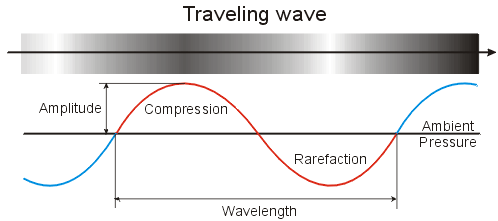
\includegraphics[width=1\textwidth, height=\textheight, keepaspectratio]{Wavelength}
	\caption[Traveling Wave]{
		Source: https://method-behind-the-music.com/mechanics/physics/ }
\end{figure}

\subsubsection{Pitch}
In music, the pitch tells how low or high a note is. In physics, it's measured in a unit called Hertz (Hz) and is called frequency. A note that vibrates at 256Hz will be caused by a sound wave vibrating at 256 times/second. \par

The speed is influenced by the medium in which it travels. Under standard temperature and pressure sound travels at 343 meters per second. \cite{speed_of_sound}

The equation (5) can be rewritten as:
\begin{equation}
Frequency = \dfrac{Speed}{Wavelength}
\end{equation}

\subsubsection{Rhythm}
